\chapter{The finite element method for elliptic problems}
\label{ch:elliptic2}

\section{The weak formulation and the finite element formulation}

We are now in position to analyze the finite element method
for an elliptic problem in detail and provide rigorous estimates
on the numerical accuracy. We remember the strong formuation:  
Find the solution $u$ of the problem

\begin{eqnarray}
\label{chp3:elliptic}
-\nabla\cdot(k\nabla u)  &=& f \quad \textrm{in}\ \Omega,\\
\label{chp3:Dirichlet}
u&=& g \quad \textrm{on}\ \partial\Omega_D, \\
\label{chp3:Neumann}
k \frac{\partial u}{\partial n}&=& h \quad \textrm{on}\ \partial\Omega_N , 
\end{eqnarray}
where we assume $\partial \Omega = \partial \Omega_D \cup \partial \Omega_N$ 
and $\partial \Omega_D \cap \partial \Omega_N = \emptyset$.

In order to arrive at the weak formulation, we introduce two Sobolev spaces
\begin{align}
H^1_{0, D} (\Omega) &= \{ u \in H^1(\Omega)  | \  T u = 0 \mbox{ on } \partial \Omega_D \}, \\   
H^1_{g, D} (\Omega) &= \{ u \in H^1(\Omega)  | \  T u = g \mbox{ on } \partial \Omega_D \}  .  
\end{align}
Here, both spaces are subspaced of the $H^1$ space introduced in the previous chapter. The 
subspaces include only the functions with appropriate values on the Dirichlet part of the boundary $\partial \Omega_D$.  
As detailed in Chapter \ref{elliptic}, we obtain the weak formulation by 1) multiplying
the equation \eqref{chp3:elliptic} with a test function $v$, 2) employing Gauss-Green's lemma, and 3) employing the 
boundary conditions. 

We arrive at the following \emph{weak formulation}, which includes the precise definitions of spaces of the trial and test functions, source function and boundary conditions: \\
Given $f\in H^{-1}_D(\Omega)$, $h\in H^{-1/2}(\partial \Omega_N)$,  
find $u\in  H^1_{g, D} (\Omega)$ such that  
\begin{equation}
\label{chp3:weak} 
\int_\Omega (k \nabla u) \cdot \nabla v \, dx = \int_\Omega f v \, dx + \int_{\partial \Omega_N} h v \, ds, \quad    \forall v\in  H^1_{0, D} (\Omega).  
\end{equation} 
Here, the negative norms are similar to the negative norms introduced in the previous chapter, although we there had Dirichlet conditions
on the complete boundary. Alternatively, and perhaps simpler from a mathematical point of view is to define it in terms of duality as
in Remark \ref{dualnorm}. When implementing the method, we seldom need to pay attention to what space our source and boundary condition functions reside in, but we remark
that it is sometimes useful to include functions that are not defined in points but only through integration over elements.  

In order to define a finite element method, let $\Omega_h$ be a mesh covering $\Omega$, consisting of a set $E_h$ of cells. 
For simplicity, we assume that the cells are simplices (triangles in 2D, tetrahedrons in 3D). Simplices 
fit very well with standard polynomials, so let ${\cal P}_k$ be the space of 
polynomials of order $k$, i.e., a basis in 2D could be $\{x^i y^{j} \}_{i,j | i+j \le k}$.   
A corresponding finite element method consist of some trial and test spaces 
\begin{align}
V_{h, 0}  &= \{ u \in H^1_{0,D}(\Omega) \ | \  \forall e \in E_h, u|_e \in {\cal P}_k \}, \\   
V_{h, g}  &= \{ u \in H^1_{g,D}(\Omega) \ | \  \forall e \in E_h, u|_e \in {\cal P}_k \} .  
\end{align}
\kent{perhaps instead introduce Lagrange elements} 
The corresponding finite element formulation is then: \\ 
Given $f\in H^{-1}_D$, $h\in H^{-1/2}(\partial \Omega_N)$,  
find $u_h\in  V_{h, g} $ such that  
\begin{equation}
\label{chp3:fem} 
\int_\Omega (k \nabla u_h ) \cdot \nabla v_h \, dx = \int_\Omega f \, v_h \, dx + \int_{\partial \Omega_N} h \, v_h \, ds, \quad    \forall v\in  V_{h, 0} .  
\end{equation} 


\section{What is an elliptic equation ? }

An elliptic partial differential equation is \emph{stricktly positive} with respect to some inner product. 
In order to show that \eqref{chp3:weak} is elliptic, we will need three concepts: Poincare's inequality, lifting, the positivity of $k$. 




Lifting, which is often used for theoretical purposes but seldom in implementation, 
refers to changing the problem from having non-homogenous Dirichlet conditions to homogenous Dirichlet conditions.  
Let us assume that $G$ is a function in $H^1(\Omega)$ such that $T u |_{\partial \Omega_D} = g$. 
Clearly, there are infinitely many such functions and in many cases it easy to find such a $G$. 
Then, by linearity, 
$u= u_0 + G$ solves \eqref{chp3:elliptic}--\eqref{chp3:Neumann} with $u_0$ defined as     
\begin{eqnarray}
\label{chp3:elliptic:lift}
-\nabla\cdot(k\nabla u_0 )  &= f +\nabla\cdot(k\nabla G)  &\quad \textrm{in}\ \Omega,\\
\label{chp3:Dirichlet:lift}
u_0&= 0 &\quad \textrm{on}\ \partial\Omega_D, \\
\label{chp3:Neumann:lift}
k \frac{\partial u_0}{\partial n}&= h - k \frac{\partial G}{\partial n} &\quad \textrm{on}\ \partial\Omega_N . 
\end{eqnarray}
Hence, the purpose of the lifting is clear: It transforms a problem with non-homogenous Dirichlet conditions, in which the Poincare's lemma
cannot be applied, to a problem with homogenous Dirichlet conditions where Poincare's lemma can be applied. It is used for theoretical purposes, 
but since $G$ can be choosen arbitrarily as long as it fit the boundary conditions, the procedure do not impose significant constraints on
the analysis. Most analysis therefore only deals with the case of homogenous Dirichlet conditions (see e.g.~\cite{braess2007finite} for more 
detailed coverage). 

In order for \eqref{chp3:elliptic} (or \eqref{chp3:elliptic:lift}) to be an elliptic problem, with  $k(x) \in \mathbb{R}^{d\times d}$ given $\Omega\in \mathbb{R}^d$,  
$k$ needs to be stricktly positive and bounded for all $x\in \Omega$. That is: \\  
For $\forall \xi\in \mathbb{R}^n$ and $\forall x \in \Omega$ there exists a $k_0 > 0$ and $k_1 < \infty$ such that 
\[
	k_0 |\xi|^2  \le    \xi^T k(x) \, \xi \le k_1 |\xi|^2 .   
\]

Given that Poincare's inequality applies and that $k$ is stricktly positive and bounded as defined above, then 
\[
\int_\Omega (k \nabla u) \cdot \nabla v \, dx 
\]
defines an inner product
on $H^1_{0, D} (\Omega)$. 
The result is crucial in this book and is hence left as a series of Exerceises \ref{ex:bilinear}--\ref{ex:poincare3}.  
The exercises show that
\begin{align}
	&\int_\Omega (k \nabla u) \cdot \nabla v \, dx,  \\  
	&\int_\Omega (\nabla u) \cdot \nabla v \, dx,  \\ 
	&\int_\Omega u v + (k \nabla u) \cdot \nabla v \, dx,  \\ 
	&\int_\Omega u v + ( \nabla u) \cdot \nabla v \, dx .  
\end{align}
are all equivalent inner products on $H^1_{0, D}(\Omega)$ . 

\section{An \emph{a priori} Error Estimate}

In the previous chapter we listed some approximation properties of polynomials in general. We will now employ these results in order to
derive \emph{a priori} error estimates. To achieve this we will need that the equation is elliptic and in addition 
the concept of Galerkin orthogonality. 


Inner products are extraordinary useful as they introduce a geometry of the space. For instance, 
a function may be orthogonal to another function. This leads us to our fourth concept: 
Galerkin orthogonality. The concept is simple, let the numerical error be $e_h = u - u_h$. Then we
remark that $v_h \in V_{h,g} \subset H^1_{g, D}$. Hence, letting 
$v=v_h$ in \eqref{chp3:weak} and subtracting \eqref{chp3:fem} we obtain:   
\begin{equation}
\label{chp3:orth}
	\int_\Omega (k \nabla (u -  u_h)) \cdot \nabla v_h \, dx = \int_\Omega (f -f) \, v_h \, dx + \int_{\partial \Omega_N} (h -h)  \, v_h \, ds = 0 \quad    \forall v\in  V_{h, 0} .  
\end{equation}
That is, the numerical error $e_h = u - u_h$ is orthogonal to all test functions $v_h$ used by the finite element method. This is a strong result and
perhaps surprising. The solution $u_h$, found by solving \eqref{chp3:fem} is therefore the best possible solution that can be found in $V_{h, g}$.   

Since, $\int_\Omega (k \nabla u) \cdot \nabla v \, dx$ defines an inner product and associated norm, equivalent with 
the standard $H^1_0$ norm we can employ the approximation result \eqref{bramblehilbert} Chapter \ref{chap-sobolev}. 
The results is called Cea's lemma, and we will later see it in a more general context. 
Here, we briefly prove an error estimate. First, we remark that, as found in the Exercises below  
\[
k_0 \int_\Omega (\nabla u)^2  \, dx \le   \int_\Omega (k \nabla u) \cdot \nabla u \, dx \le   
k_1 \int_\Omega (\nabla u)^2  \, dx,  \\  
\]
As such 
\begin{align*}
	k_0 \int_\Omega (\nabla (u-u_h))^2  \, dx &\le   \int_\Omega (k \nabla (u -u_h)) \cdot \nabla (u-u_h) \, dx \\    
&\le   \int_\Omega (k \nabla (u -u_h)) \cdot \nabla (u-P_m u + P_m u - u_h) \, dx, \\ 
&\le   \int_\Omega (k \nabla (u -u_h)) \cdot \nabla (u-P_m u ) \, dx \\ 
&\le   k_1 \int_\Omega (\nabla (u -u_h)) \cdot \nabla (u-P_m u ) \, dx 
\end{align*}
Here, we use that we may subtract and add $P_m u$ which totals to zero, and remark that both $u_h$ and $P_m u$ 
are in $V_{h,0}$ and hence both are orthogonal to $u - u_h$ as in \eqref{chp3:orth}. 
Further, by using Cauchy-Schartz inequality, which in this case states that   
\begin{align*}
&  \int_\Omega ( \nabla (u -u_h)) \cdot \nabla (u-P_m u ) \, dx \\ \le  
&  
(\int_\Omega ( \nabla (u -u_h))^{2} dx )^{1/2} \,  (\int_\Omega \nabla (u-P_m u )^2 \, dx)^{1/2} 
\end{align*}
we immediately have by the Bramble-Hilbert lemma \eqref{bramblehilbert} that 
\begin{align}
(\int_\Omega ( \nabla (u -u_h))^{2} dx )^{1/2} \le \frac{k_1}{k_0}   (\int_\Omega \nabla (u-P_m u )^2 \, dx)^{1/2} 
 \le \frac{k_1}{k_0}  C h^{m-1} |u|_{m} 
\end{align}

\begin{example}{Estimating the convergence rate}
\label{ex:poisson1d}
Let us consider the Poisson problem, $-\Delta u = f$, on the unit interval 
with homogenuous Dirichlet conditions with a manufactured solution
$u = \sin(k \pi x)$ such that we can check the convergence rate. Let us
consider the Lagrange element of various orders. From the above Cea's lemma we an error rate of $m$ in the $H^1$-seminorm.  
The following code implements a solver and estimates the rates. 
\begin{python}
from dolfin import * 

def boundary (x): return x[0] < DOLFIN_EPS or x[0] > 1 -DOLFIN_EPS 

f = Expression("M_PI*M_PI*sin(M_PI*x[0])", degree=P+5)
u_analytical = Expression("sin(M_PI*x[0])", degree=P+5)

Ns = [4, 8, 16, 32, 64, 128, 256]
Ps = [1, 2, 3, 4]
L2_errors = {} 

for P in Ps: 
    for N in Ns: 
        mesh = UnitIntervalMesh(N) 
        h = mesh.hmax()
        V = FunctionSpace(mesh, "Lagrange", P) 
        u = TrialFunction(V) 
        v = TestFunction(V) 

        # bc 
        u0 = Constant(0)
        bc = DirichletBC(V, u0, boundary) 

        a = inner(grad(u), grad(v))*dx  
        L = f*v*dx 

        U = Function(V) 
        solve (a ==L, U, bc) 

        L2_error = assemble(pow(U-u_analytical, 2)*dx) 
        L2_error = sqrt(L2_error) 

        L2_errors[(P, N)] = (h, L2_error)  

# numbers to estimate the rates 
for P in Ps: 
    for i in range(len(Ns)-1):  
        print ("P ", P, L2_errors[(P, Ns[i])][1] / L2_errors[(P, Ns[i+1])][1])


# log-log plot for assessing whether the convergence rate is 
# polynomial and what the rate is 
from numpy import log
import matplotlib.pyplot as plt
for P in Ps: 
    hs = []
    errors = []
    for N in Ns: 
        h, error = L2_errors[(P, N)]
        hs.append(h)
        errors.append(error)
    plt.loglog(Ns, errors)
plt.show()
\end{python}
In Fig.~\ref{fig:poisson1D:rates} we show a log-log plot of the error for different mesh resolutions and element orders. The linear relationship shows that the 
error behaves in a polynomial fashion, except for the case with very small errors where we see stagnation due to round of errors. 
We remark that we assess the error in $L^2$ which rather than the $H^1$. By inspection, we notice that the error rate is $m+1$, i.e. second order for linear elements. 
\end{example} 

\begin{figure}
\begin{center}
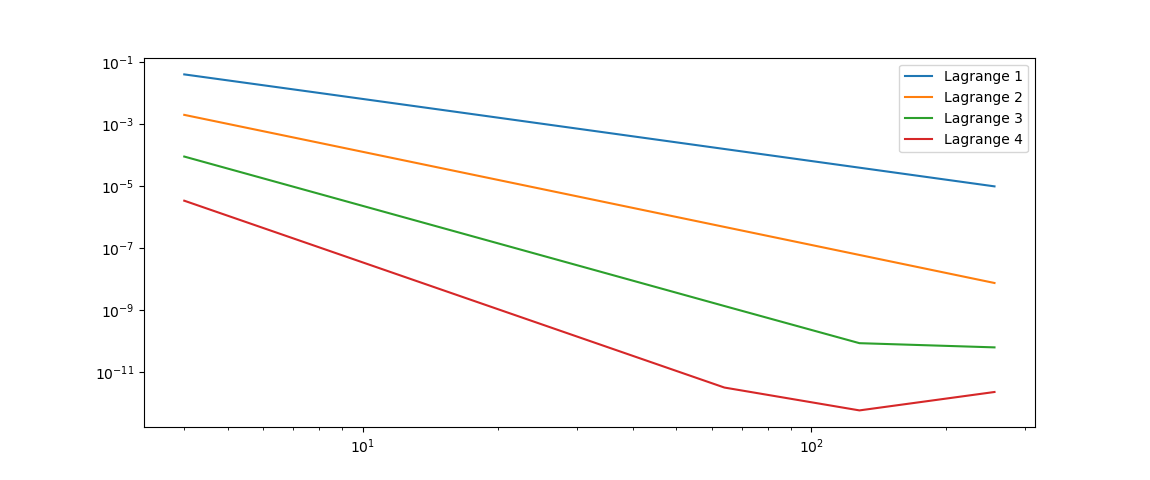
\includegraphics[width=0.95\textwidth]{chapters/elliptic2/plots/poisson1d.png}
\caption{The error for Lagrange elements of various orders in a log-log plot.  
The log-log plot shows a clear linear relationship for the various orders demonstrating polynomial order.   
}
\label{fig:poisson1D:rates}
\end{center}
\end{figure}



\section{Exercises}

\begin{exercise}
\label{ex:bilinear}
Let $\Omega=(0,1)$.  
Show that 
\[  
a(u, v) = \int_\Omega  u \, v \, dx 
\]
is a bilinear form. 
\end{exercise}

\begin{exercise}
\label{ex:inner}
Let $\Omega=(0,1)$.  
Show that 
\[  
a(u, v) = \int_\Omega  u \, v \, dx 
\]
forms an inner product.  
\end{exercise}




\begin{exercise}
\label{ex:poincare}

Let $\Omega=(0,1)$ then  
for all functions in $H^1_0(\Omega)$ then
Poincar\'e's inequality states that
\[
|u|_{L^2} \le C  |\frac{\partial u}{\partial x}|_{L^2}   
\]
Use this inequality to show that the $H^1$ semi-norm defines 
a norm equivalent with the standard $H^1$ norm on $H^1_0(\Omega)$.  
\end{exercise}



\begin{exercise}
\label{ex:poincare2}

Let $\Omega=(0,1)$.  
Show that 
\[  
a(u, v) = \int_\Omega \nabla u \cdot \nabla v \, dx 
\]
forms an inner product on $H^1_0(\Omega)$  equivalent with the standard
$H^1(\Omega)$ inner product. 
\end{exercise}

\begin{exercise}
\label{ex:poincare3}

Let $\Omega=(0,1)$.  
Show that 
\[  
a(u, v) = \int_\Omega k \nabla u \cdot \nabla v \, dx 
\]
forms an inner product on $H^1_0(\Omega)$ given that $k \in \mathbb{R}^{n \times n}$ is stricktly positive
and bouded. The inner product is equivalent with the $H^1_0(\Omega)$ inner product.  


\end{exercise}



